\documentclass[12pt]{article}
\usepackage[top=1in,bottom=1in,left=1in,right=1in]{geometry}

\usepackage[english]{babel}
\usepackage[utf8x]{inputenc}
\usepackage{mathtools}
\usepackage{amsmath}
\usepackage{graphicx}
\usepackage{float}
\setlength{\parskip}{12pt}

\title{3D Color Model Reconstruction by Using the Kinect}
\author{ \parbox{3.5 in}{\centering Peng Liu\\
    {\tt\small liux1342@umn.edu}\\
  Department of Computer Science}
}
\date{ }
\begin{document}
\maketitle

\begin{abstract}
3D color models of the real world, such as indoor scenes, the human  body and objects around  our daily life, are useful for applications in computer games,  animation and  virtual  reality. Accurate model recreation systems, however, either require very expensive scanners or require tedious effort using modeling software. Cheap depth  sensors like the Microsoft Kinect,  which have the potential to facilitate the model creation task, have attracted tremendous attention in academia. However, most research efforts have been aimed at doing pose tracking or robotic navigation, and few have focused on using these depth sensors to do color model reconstruction. In this paper we present such a depth sensor based system, which uses a Kinect to do color model reconstruction. The system uses an incremental updating scheme based on the KinectFusion algorithm\cite{Newcombe2011}. With this fast and affordable color modeling system (only a Kinect and decent graphic card are needed), creating real world objects can be done more easily than before, which promises a more efficient development process in model creation related applications.
\end{abstract}

\section{Introduction}
In many computer graphics related applications, like animation, video games or even research areas like virtual reality and augmented reality, the task of creating a realistic model is either performed by graphics specialists, who employ specialized design software, or by using a 3D scanning system to capture a real object. Either way, the work is expensive (both the advanced design software and the scanner are expensive) and time consuming.

Recently, the invention of the Kinect, a cheap depth sensor, has drawn extensive attention in both industry and academia. Compared with conventional 3D scanners, which are capable of capturing depth and image data at video rate, the Kinect is more compact, cheaper and easier to use. Thus, some research groups have tried to use the Kinect as a 3D scanner. However, many of these applications (especially those that only use a few frames from the depth sensor) suffer from the comparably low resolution and depth accuracy of the depth sensor; therefore, numerous efforts have been put into increasing the quality of the depth image. For example, Sun \textit{et al.}\cite{Sun2012} proposed an automatic face modeling system which uses the Kinect to do high resolution 3D facial modeling. In order to address the issue of low quality depth data, they built a resolution enhancement framework that uses image segmentation and smoothing techniques to capture a high resolution partial face model. Cui \textit{et al.}\cite{Cui2013} describe a method to improve the quality of the incoming depth map through a super resolution algorithm which takes several low resolution depth images of the target from the same view port and outputs one high resolution depth image. Weiss \textit{et al.}\cite{Weiss2013} presented a system to perform 3D body scans from a single Kinect, circumventing the low quality depth image problem by using a human body template. Their system takes several depth snapshots of a target human body, then based on the silhouette of each snapshot, their system finds the body pose by fitting a template body onto the silhouette, and updates each partial model of the human body according to the pose of each part of the template body. 

The aforementioned systems only use a single Kinect to capture target models, and all have some limitations: Sun's system can only generate partial facial models; Weiss's system does not account for subjects' clothing; and Cui's system takes a long time to process and requires a rotating disk, which further limits its applications. To extend the usage of the Kinect, some researchers try to use multiple Kinects working together to get better results. Tong \textit{et al.}\cite{Tong2012} created a multi-Kinect based body scanner. Their system uses three fixed Kinects looking at different, non-overlapping parts of the human body. The target needs to stand on a fixed turntable for a 360 degree scan before the system can output the complete model of the human body. A major limitation of their system is that it can only create models of objects that can be put onto the turntable. The system also requires a setup process that further limits its applicability. The above systems all have a limitation in that they have separated the capturing phase and the processing phase, which is disadvantageous for real-time applications, such as immersive virtual reality. To address this issue, Alexiadis and his team\cite{Alexiadis2013} developed a system that uses multiple Kinects to do real-time full 3D reconstruction of objects. Their system receives multiple depth data streams from multiple Kinects through different viewpoints, applies a coarse-to-fine registration algorithm to register different partial surfaces of the target, and merges separate meshes into a single 3D surface. However, due to the high noise level of the live depth map from the Kinect, the quality of their generated mesh is hardly acceptable for immersive virtual reality applications. 

A great leap in depth sensor based scanning systems was made in 2011, when Newcombe \textit{et al.}\cite{Newcombe2011} introduced the KinectFusion algorithm, which uses a dense mapping approach to register consecutive depth maps, and then fuses the incoming depth surfaces into a truncated distance volume for model generation. That was the first real-time dense model fusing system with unprecedented accuracy. It is truly remarkable that with just one hand-held depth sensor, their system can produce a very accurate geometric model. However, their system cannot do a full color model reconstruction, and due to their implementation decisions, their system can only work on systems with an Nvidia Graphics card with the CUDA feature installed.  In this paper, we present a system based on the KinectFusion algorithm, which uses both the depth data stream and the RGB data stream to create a color model of any object or indoor scene without relying on any CUDA implementation.


\section{Approach}
In this section we describe our system in detail. The framework of our system consists of several key processing steps: raw data acquisition, preprocessing, surface extraction, surface alignment, volume updating and visualization --- see Figure~\ref{fig:framework} for information about the system work-flow. In the following subsection we will explain each key step.

\begin{figure}[h!]
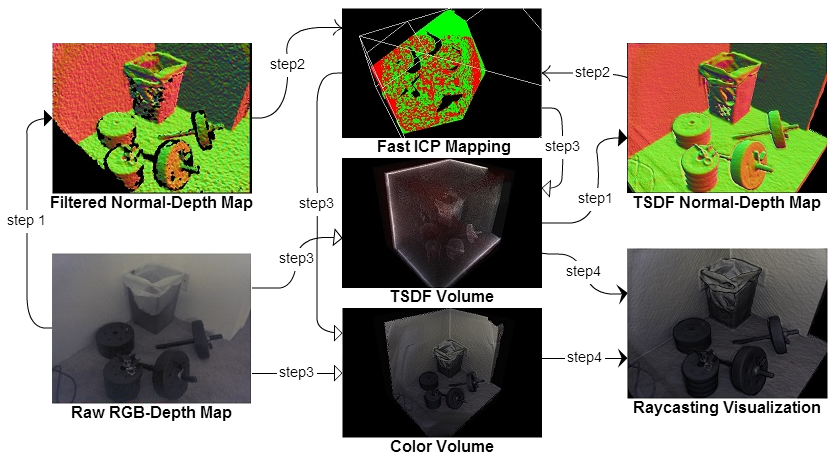
\includegraphics[width=\textwidth]{work-flow.png}
\caption{\label{fig:framework}The overall system work-flow. After each new raw RGB-Depth map has been received, the system will perform an operation sequence to integrate the new data into the implicit target model representation -- the TSDF volume (a 3D grid based model representation, we'll explain it in detail in later section). In step 1, raw data will be filtered to get rid of noise, then a normal-depth map will be generated. At the same time, another normal-depth map will be extracted from the TSDF volume for mapping. In step 2, the fast ICP algorithm (an algorithm used to register two normal-depth maps, explained in later section) will find the rigid transform matrix between two normal-depth maps to get the pose of the Kinect. In step 3, with the transform matrix and the raw RGB-Depth data, both the TSDF and the Color volume will be updated to incorporate the new measured surface. Then in step 4, a ray-casting algorithm will sample both the TSDF and the Color volume to generate a Phong shaded image of the target model}
\end{figure}

\subsection{RGB-Depth acquisition}
The Kinect has a structured light-based depth sensor along with a commodity RGB camera. The depth sensor is capable of generating a 640x480 depth map at 30 frames per second. At each frame, the Kinect will stream out both the depth map and the RGB image; in order to reconstruct the color 3D model, the depth map and the color image must be registered. However, the offset between the RGB sensor and the depth sensor makes it impossible to correctly register the depth and RGB map for all depth levels, so artifacts will appear around the edges when assigning colors to the model. Our system addresses this problem by simply not updating colors near edges. However, when we have small objects very near the sensors, such as cables in front of the Kinect, the color artifacts can still appear. A more sophisticated method may be developed in the future to address this issue.

\subsection{Pre-Processing}
With the low cost of the Kinect, the quality of the depth sensor is acceptable, but there are still some challenges for the Kinect to do an accurate 3D scan. One major problem is the high noise level of the depth data. The Kinect was mainly designed to track human body movement from 1 to 4 meters away, so the high noise level would not affect the result too much. But for reconstructing a model with fine details, noisy depth data causes problems. Although we could average out the noise by using multiple scans for one surface measurement, the pose estimation phase (finding the rigid body transformation to register two depth maps) will be badly affected by this noise. To get an accurate pose estimation, our system applies a bilateral filter on each incoming depth map to remove the noise, while at the same time keeping the sharp edges of the depth map (the surface discontinuities must be kept to correctly reconstruct the geometry). The bilateral filter adopted in our system is the separable version, in which the 7x7 kernel pass was separated into two 1x7 (horizontal and vertical) kernel passes. To maintain real-time performance, we utilize the power of the GPU by performing the filter algorithm purely on the GPU using a pixel shader. The filtered depth map was only used for pose estimation (in the Fast ICP process), while during the updating phase, the raw RGB-Depth data was used instead, in order to keep the high frequency detail.

\subsection{Surface alignment}
The correctness of incremental model updating is ensured by aligning the incoming partial surfaces with the model surface we already have. This problem has been well studied in robotics as SLAM (simultaneous localization and mapping), and the most popular solution to align 3D surfaces based on geometry information (with initial estimate pose known) is the ICP (iterative closest point) algorithm. After the introduction of the ICP algorithm, many variants have been developed. Rusinkiewicz and Levoy \cite{Rusinkiewicz} provide a well organized review and efficient comparison of some of the most popular variants of the ICP algorithm. In Rusinkiewicz's review, there are basically six stages in the ICP algorithm: selection; matching; weighting; rejecting; error metric assignment; and error metric minimizing. Most ICP variants differentiate from each other by using a different method in at least one stage of the ICP algorithm routine. According to their research and our system specification, we chose two different ICP algorithms as candidates. Both use all available points during the selecting phases, and use the same criteria for the rejecting and weighting phases; one uses the modified nearest point algorithm for matching and point-to-point distance as the error metric, the other uses projecting rays for point matching and point-to-plane distance as the error metric. The reason behind our decision is that \cite{Rusinkiewicz} suggests that the point-to-point method has a lower execution time per iteration, while the point-to-plane method, although it has a longer per iteration execution time, has a better convergence rate, which means that it will iterate for less time to get the result. 

\begin{figure}[h!]
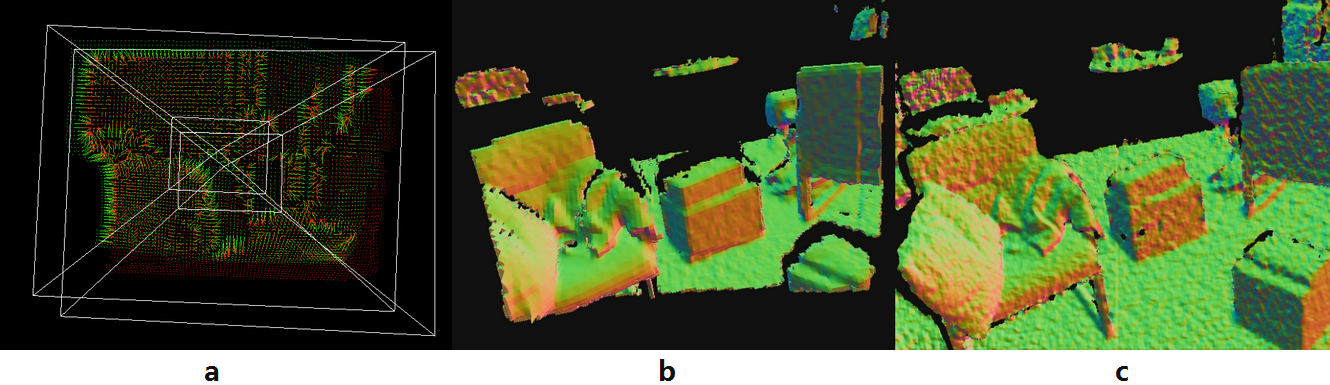
\includegraphics[width=\textwidth]{point_to_point_matching.png}
\caption{\label{fig:point_to_point}(a) demonstrates the closest corresponding matching phase, in which every green point will search on a neighbor area in the red point cloud to find the closest corresponding point, which is very time consuming even when implemented on the GPU. (b) shows the normal shaded model that was reconstructed, while (c) shows the live depth map at that time. There is nearly 2 seconds delay during the updating phase, thus the point-to-point version of our system cannot currently achieve real-time performance, but with more powerful hardware it may}
\end{figure}

The point-to-point method we tried used a modified closest point matching strategy, in which each point searched for a closest point around it in the target depth map instead of in the whole depth map. Our result shows that in order to allow 3 degrees of rotational movement between neighbor depth maps (it is quite common that we can rotate the Kinect by hand about 3 degrees in $1/30$ second), the search area in a typical 640x480 depth map has to be at least 50x50. Even a sample rate of just $0.25^2$ (for every 4x4 points, sample only 1 point) will require 100 iterations for each vertex, and our system can only get 7 FPS on such a setting. So actually the point-to-point version cannot achieve real-time performance. See Figure~\ref{fig:point_to_point} for details.

\subsubsection{Fast ICP alogrithm}
The point-to-plane iterative correspondent point variant is actually called Fast ICP, introduced by Chen and Medioni \cite{Chen1991}. The differences between their algorithm and the standard ICP are in how they do point matching and in the error metric they use. As shown in Figure~\ref{fig:ICP_matching}, the Fast ICP method uses a projection ray from the viewpoint to find a matching point on the target surface while the standard version's matching routine searches for the closest point on the whole target surface. 

When having two depth maps in hand, the matching phase is quite simple: since the two depth maps have the same resolution, following the projective association algorithm, the corresponding point pair actually have same texture index (we implement this algorithm in the form of a pixel shader, and we pass the two depth maps into the pixel shader as texture objects). So actually there is no computational cost in the matching phase.

\begin{figure}[h!]
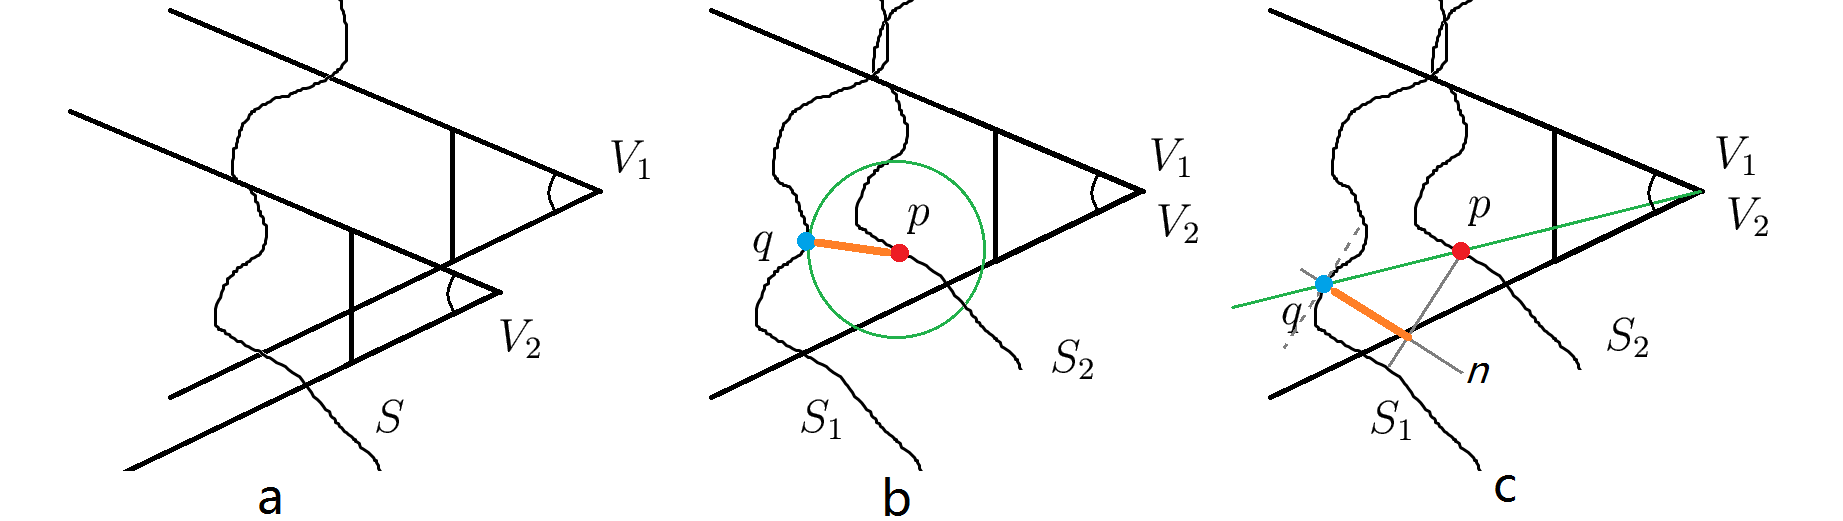
\includegraphics[width=\textwidth]{ICP_matching.png}
\caption{\label{fig:ICP_matching}Demonstration of the differences in the matching stage of the standard ICP algorithm and the Fast ICP algorithm used in our system. In (a) we measure a surface $S$ from different viewpoints $V_1$, $V_2$ and get the surface measurement $S_1$, $S_2$. In (b) we demonstrate the standard ICP matching strategy: for point $p$ in $S_2$, the corresponding point $q$ is the closest point to $p$, and the error is the distance between $p$ and $q$. In (c) the Fast ICP uses the projective data association algorithm \cite{Chen1991} to obtain the correspondent point $q$, and the error is the distance between $p$ and the tangent plane of $q$ }
\end{figure}

However, the Fast ICP algorithm uses a point-to-plane error metric for the final minimizing stage (Equation~\ref{point_to_plane}, where $R$ is the rotation matrix, $t$ is the translation vector, and $n$ is the normal vector at point $q_i$) which is more complex than the standard point-to-point error metric version (Equation~\ref{point_to_point}) and requires the knowledge of its normal map. See Figure~\ref{fig:ICP_matching} for details.
\begin{equation}\label{point_to_plane}
E=\sum_{i}{}\big[(Rp_i+t-q_i)\cdot n_i\big]^2
\end{equation}
\begin{equation}\label{point_to_point}
E=\sum_{i}{}(Rp_i+t-q_i)^2
\end{equation}
The normal map for the Fast ICP algorithm is generated by calculating the cross product of the two edge vectors consisting of the current point and its two neighbor points. The result of our system shows that the increased workload of the Fast ICP algorithm is offset by the reduced iterations and it actually achieves real-time performance.

\subsubsection{Pose estimation}
The Kinect's initial 6DOF pose is defined as centered at $( 0, 0, 0 )$ looking along the positive $z$ axis in global space, so the pose of the $k$th depth frame is defined by a transformation matrix
$$T_k = \begin{bmatrix}
            R_k         &   \mathbf{t_k} \\
            \mathbf{0}   &   1           
        \end{bmatrix}$$
where the $R_k$ is a 3x3 rotation matrix and $\mathbf{t_k}$ is the translation vector. This matrix maps the surface in the Kinect's local space onto the global space. Thus every measured point $p$ in local space can be transformed into global space as $\mathbf{p_g} = T_k\mathbf{p_k}$.

The depth map is actually a one-channel image, and each texel $(u,v)$ only stores the $z$ axis distance from the nearest surface to the depth sensor $D(u,v)$. In order to get the 3D coordinate of each point $V(p)$ in the depth map, another back projection matrix is needed. Once we know the intrinsic camera calibration parameters, we can build the function
$$V\big(D(u,v)\big)=\Big(\frac{(u-c_u)D(u,v)}{f_u},\frac{(v-c_v)D(u,v)}{f_v},D(u,v)\Big)$$
to map the surface measurement $D(u,v)$ to the actual 3D point $V\big(D(u,v)\big)$ in local space ($c_u,c_v$ are the $u,v$ indices of the center point in the depth texture, while $f_u,f_v$ are the focal length).

The Kinect pose transformation matrix in frame $k$ is the one that aligns the $k$th measured surface with the global reference model. So with two point clouds (surfaces) in hand, we can get the rigid-body transformation matrix by solving an optimization problem that is aimed at finding the optimal matrix $R$ and vector $t$ to minimize the alignment error. The error metric used in our system as mentioned above is the point-to-plane distance, so with a collection of points $(p_i,q_i)$ and normals $n_i$, we need to minimize the point-to-plane alignment error
$$
E = \sum_{i}{}\big[(Rp_i+t-q_i)\cdot n_i\big]^2
$$
where $R$ is the rotation matrix and $t$ is the translation vector. Since there are trigonometric functions in the rotation matrix, this optimization system is nonlinear. However, it is possible to linearize this system by utilizing the fact that the rotational movement will be very small between two consecutive frames, since we are hand-holding the Kinect. So it is safe to approximate $cos\theta$ as 1 and $sin\theta$ as $\theta$. Then our rotation matrix $R$ can be approximated as
\begin{equation}\label{rotation_matrix}
    \begin{split}
        R &= R_{x,\alpha}\times R_{y,\beta}\times R_{z,\gamma}\\
          &=
        \begin{bmatrix*}[r]
            1   &   0           &   0           \\
            0   &   cos\alpha   &   -sin\alpha  \\
            0   &   sin\alpha   &   cos\alpha
        \end{bmatrix*}
        \begin{bmatrix*}[r]
            cos\beta    &   0   &   sin\beta    \\
            0           &   1   &   0           \\
            -sin\beta   &   0   &   cos\beta
        \end{bmatrix*}
        \begin{bmatrix*}[r]
            cos\gamma   &   -sin\gamma   &   0  \\
            sin\gamma   &   cos\gamma    &   0  \\
            0           &   0            &   1
        \end{bmatrix*}\\
        &\approx
        \begin{bmatrix*}[r]
            1       &  -\gamma  &   \beta   \\
            \gamma  &  1        &   -\alpha \\
            -\beta  &  \alpha   &   1
        \end{bmatrix*}
    \end{split}
\end{equation}
for rotations $\alpha$, $\beta$ and $\gamma$ around axis $x$, $y$ and $z$.

Substituting \eqref{rotation_matrix} into \eqref{point_to_plane}, and rewriting some terms we obtain
\begin{equation}\label{energy_func_expanded}
E = \sum_{i}{}\big[(p_i-q_i)\cdot n_i +t\cdot n_i+\alpha(p_{i,y}\cdot n_{i,z}-p_{i,z}\cdot n_{i,y})+\beta(p_{i,z}\cdot n_{i,x}-p_{i,x}\cdot n_{i,z})+\gamma(p_{i,x}\cdot n_{i,y}-p_{i,y}\cdot n_{i,x})]^2
\end{equation}
Defining $r=[\alpha,\beta,\gamma]$, and simplifying \eqref{energy_func_expanded} we get the alignment error function as
$$E = \sum_{i}{}\big[(p_i-q_i)\cdot n_i+t\cdot n_i+r\cdot (p_i\times n_i\big)]^2$$
To minimize $E$ with respect to $\mathbf{r}$ and $\mathbf{t}$(specifically: $\alpha,\beta,\gamma,t_x,t_y,t_z$), we set the partial derivatives to zero:
\begin{equation}
    \begin{split}
        &\frac{\partial E}{\partial \alpha} = \sum_{i}{}2(p_i\times n_i)_x\big[(p_i-q_i)\cdot n_i+r\cdot (p_i\times n_i)\big] = 0\\
        &\frac{\partial E}{\partial \beta} = \sum_{i}{}2(p_i\times n_i)_y\big[(p_i-q_i)\cdot n_i+r\cdot (p_i\times n_i)\big] = 0\\
        &\frac{\partial E}{\partial \gamma} = \sum_{i}{}2(p_i\times n_i)_z\big[(p_i-q_i)\cdot n_i+r\cdot (p_i\times n_i)\big] = 0\\
        &\frac{\partial E}{\partial t_x} = \sum_{i}{}2n_{i,x}\big[(p_i-q_i)\cdot n_i+r\cdot (p_i\times n_i)\big] = 0\\
        &\frac{\partial E}{\partial t_y} = \sum_{i}{}2n_{i,x}\big[(p_i-q_i)\cdot n_i+r\cdot (p_i\times n_i)\big] = 0\\
        &\frac{\partial E}{\partial t_z} = \sum_{i}{}2n_{i,x}\big[(p_i-q_i)\cdot n_i+r\cdot (p_i\times n_i)\big] = 0
    \end{split}
\end{equation}
Defining $c_i=p_i\times n_i$ and reorganizing these equations in matrix form we get
$$
    \sum_{i}{}
    \begin{bmatrix*}
        c_{i,x}c_{i_x}&c_{i,x}c_{i_y}&c_{i,x}c_{i_z}&c_{i,x}n_{i_x}&c_{i,x}n_{i_y}&c_{i,x}n_{i_z}\\
        c_{i,x}c_{i_y}&c_{i,y}c_{i_y}&c_{i,y}c_{i_z}&c_{i,y}n_{i_x}&c_{i,y}n_{i_y}&c_{i,y}n_{i_z}\\
        c_{i,x}c_{i_z}&c_{i,y}c_{i_z}&c_{i,z}c_{i_z}&c_{i,z}n_{i_x}&c_{i,z}n_{i_y}&c_{i,z}n_{i_z}\\
        c_{i_x}n_{i,x}&c_{i_y}n_{i,x}&c_{i_z}n_{i,x}&n_{i,x}n_{i_x}&n_{i,x}n_{i_y}&n_{i,x}n_{i_z}\\
        c_{i_x}n_{i,y}&c_{i_y}n_{i,y}&c_{i_z}n_{i,y}&n_{i,x}n_{i_y}&n_{i,y}n_{i_y}&n_{i,y}n_{i_z}\\
        c_{i_x}n_{i,z}&c_{i_y}n_{i,z}&c_{i_z}n_{i,z}&n_{i,x}n_{i_z}&n_{i,y}n_{i_z}&n_{i,z}n_{i_z}\\
    \end{bmatrix*}
    \begin{bmatrix*}
        \alpha\\
        \beta\\
        \gamma\\
        t_x\\
        t_y\\
        t_z\\
    \end{bmatrix*}
    =-\sum_{i}{}
    \begin{bmatrix*}
        c_{i,x}(p_i-q_i)\cdot n_i\\
        c_{i,y}(p_i-q_i)\cdot n_i\\
        c_{i,z}(p_i-q_i)\cdot n_i\\
        n_{i,x}(p_i-q_i)\cdot n_i\\
        n_{i,y}(p_i-q_i)\cdot n_i\\
        n_{i,z}(p_i-q_i)\cdot n_i\\
    \end{bmatrix*}
$$

To solve this linear system, we use the Cholesky decomposition. Then the result $\alpha$, $\beta$, $\gamma$, $t_x$, $t_y$, $t_z$ gives us the optimal incremental rotation and translation parameters. Thus real-time pose tracking is accomplished by repeatedly multiplying the current transformation matrix with the incremental matrix.

In our system, all per-point computation and summation is implemented as a pixel shader running on the GPU in order to get real-time performance, while the Cholesky decomposition is done by using the Eigen library on the host CPU. The target point cloud ($p_i$) is extracted from the TSDF(mentioned in the next section), while the model point cloud ($q_i$) is taken from the Kinect's depth sensor after pre-processing by the bilateral filter. The reason we don't simply use the adjacent depth map (depth maps from frame $k$ and frame $k-1$) for the pose estimation is that the alignment error will accumulate, which can cause our system to fail after several seconds.  


\subsection{Model representation and updating}

Once every new depth map gets aligned, it can be used to update the mesh model. One straightforward way to do this would be to use a mesh-based reconstruction algorithm to add all of the aligned points into the output model, but a post-trimming process is needed since in each frame there can be up to 640x480 points that need to be added in which can overload the system very quickly. On the other hand, the trimming process may also be time consuming when the model is complex, and for our pose estimation processing to work correctly, we have to ensure the small movement assumption, which means that we need to maintain a constant execution time for each frame. So the mesh-based method is not suitable for our purpose; instead, as suggested by \cite{Newcombe2011}, we use a truncated signed distance function (TSDF) to represent the model. 

The \texttt{SDF} (signed distance function) was introduced by Curless and Levoy \cite{Curless1996} who used that method to fuse partial depth scans and avoid problems related to the mesh-based method as mentioned above. Using SDF, the model is implicitly represented in a volume (a 3D grid), and each voxel in the SDF volume stores the distance to the nearest surface. The voxels that are outside the object have positive value while those inside have negative value. Thus the actual mesh is encoded as the crossing zero surface in the volume (see Figure~\ref{fig:TSDF_Representation} for details). 

In our system, we use a truncated version of the SDF to store the model. Basically, the truncated SDF defines a distance threshold, if the distance value in any voxel is greater than the threshold, that value will be set to the threshold value. For a voxel at $p=(x,y,z)$, the TSDF($V(p)$) in our system stores the truncated distance to the "nearest" surface $D_{trunc}(p)$, and a weight $W(p)$.
$$V(p) = \big[ D_{trunc}(p), W(p)\big]$$
To calculate the truncated distance for $V(p)$, we first project voxel $p$ onto the virtual Kinect's image plane (which contains the depth map $D$), using the calculated pose matrix $T_k$, and the projection matrix $M_{proj}$ to get the corresponding measured point $D(M_{proj}T_k^{-1}p)$, then we truncate the distance between $p$ and $D(M_{proj}T_k^{-1}p)$ by the predefined $TruncateDist$. The truncated distance is defined as 
\begin{equation}\label{updating}
    D_{trunc}(p)=
    \begin{cases}
        min\big(\frac{T_k^{-1}p-D(M_{proj}T_k^{-1}p)}{TruncateDist},1\big) &\text{if}~D(M_{proj}T_k^{-1}p)-T_k^{-1}p>-TruncateDist\\
        \text{null}
    \end{cases}
\end{equation}
The weight $W(p)$ is used to fuse the incoming depth data with the previous data to get a smooth surface when updating the volume. The weighting strategy used in our system initially assigns each measurement the weight 1, and truncates the resulting weight to a predefined $MAXWEIGHT$ to allow scene updating during model reconstruction. 

\begin{figure}[h!]
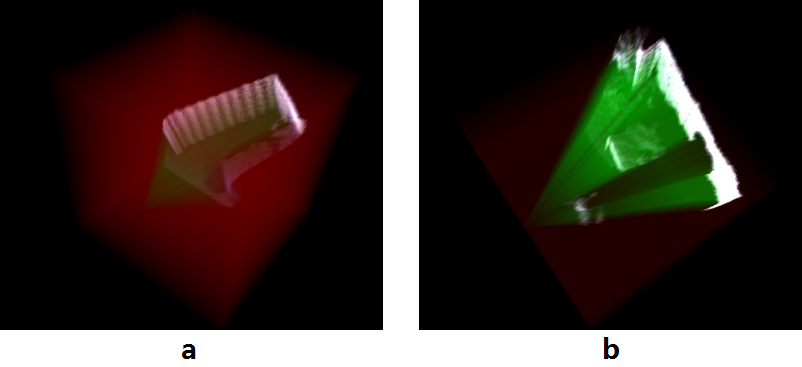
\includegraphics[width=\textwidth]{TSDF.png}
\caption{\label{fig:TSDF_Representation} Both (a) and (b) are the visualizations of the TSDF volume taken from different viewpoints. The TSDF volume is a 3D grid, the voxels in red are not being visited by the Kinect's frustum and the voxels in green represent empty space within the frustum. The remaining voxels actually contain the model surface.}
\end{figure}

The center of the TSDF volume was defined as the origin at $o(0,0,0)$ in global space. With the proper voxel size and voxel resolution settings, each voxel in this volume can be easily located. When extracting the depth map from the TSDF for pose estimation, a virtual Kinect frustum will be created and transformed to the right place by using the previous transformation matrix (see equation~\ref{updating}). Our system will then ray cast the TSDF volume through the virtual Kinect's frustum. The ray casting algorithm detects the zero crossing surface and generates a depth map for incoming surface alignment (See Figure~\ref{fig:raycasting}). So in our system, the distance value in the TSDF is not the exact distance to the nearest surface, but the distance to the nearest surface along the projection ray. However, after several scans are integrated into the TSDF, the voxels near the surface have the approximately the same distance value as to the nearest surface. So during the surface extraction phase, we only use the voxels near the surface to calculate the zero crossing interface.

While updating the TSDF volume after the pose estimation process, the same ray casting algorithm is used, with the exception that every voxel that intersects the cast rays will be updated. For each voxel position $p$ along the rays in frame $k$, the previous value in that voxel is extracted: $D_{trunc,k-1}(p),W_{k-1}(p)$. Then, with the new measured truncated distance $D_{trunc}(p)$, we update the volume by using the following formula:
$$D_{trunc,k}(p) = \frac{W_{k-1}(p)D_{trunc,k-1}(p)+D_{trunc}(p)}{W_{k-1}(p)+1}$$    
$$W_k(p) = min(W_{k-1}(p)+1,MAXWEIGHT)$$
At the same time, the color volume is also updated. As mentioned in the RGB-Depth acquisition section, we don't update those voxels that are near the silhouette of the incoming RGB-Depth map to avoid artifacts. Also, the color updating process uses the weight of the previous value in the color volume $Color_{k-1}(p)$ to avoid turbulence in the color representation:
$$Color_k(p) = \frac{W_{k-1}(p)Color_{k-1}(p)+Color(p)}{W_{k-1}(p)+1}$$    
$$W_k(p) = min(W_{k-1}(p)+1,MAXWEIGHT)$$

\begin{figure}[h!]
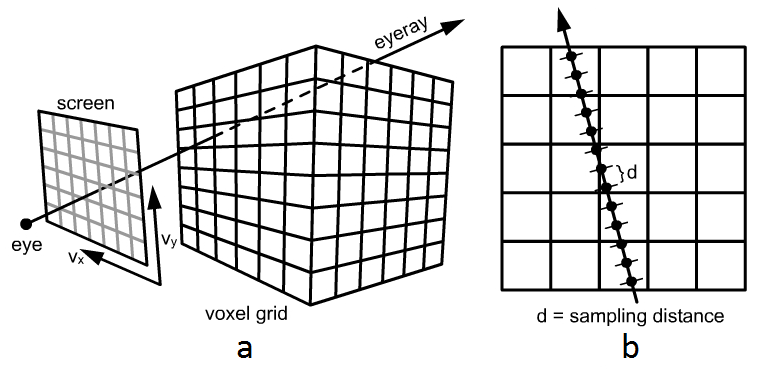
\includegraphics[width=\textwidth]{raycasting.png}
\caption{\label{fig:raycasting} (a) With known frustum pose, a projection screen (screen) and viewpoint (eye) can be uniquely located, then for each pixel in the projection screen, an eyeray will emit from eye through that pixel into the voxel grid. (b) Each eyeray will sample the volume along its way, and the surface interface is detected by finding the two neighboring samples which have a negative product (one is greater than 0 while the other is less than 0). Then a linear interpolation will find the exact crossing zero surface. (image comes from: http://johnrichie.com/V2/richie/isosurface/volume.html)}
\end{figure}

As described above, a lot of voxels will be updated (typically, in our system both the TSDF and Color volume have a size of $382^3$ voxels, and during each frame nearly 70\% of them will be updated). To maintain interactive frame rates, all of the extracting and updating phases were implemented as a pixel shader program in our system utilizing the power of the massive parallelism of the GPU. The result shows that our system can maintain a 25 FPS performance even with a $512^3$ volume size for both the TSDF and Color volume (that is 40ms per frame execution time including rendering the model from the volume), which is pretty good given the fact that the depth stream of the Kinect sensor is working at 30 FPS.

\subsection{Volume visualization}
Once the volume gets updated, visualization is very straight foreword. We define a free virtual camera in our system, and use the extracting method described above to get the rendered image from the TSDF, except that instead of passing in the tracked Kinect pose as input, we pass in the free camera's pose. Also, after finding the zero crossing point in the TSDF, we sample the color volume at the same place to get the color information for that point, then we use a Phong shading algorithm to shade the model. See Figure~\ref{fig:shading} for the result.

\begin{figure}[h!]
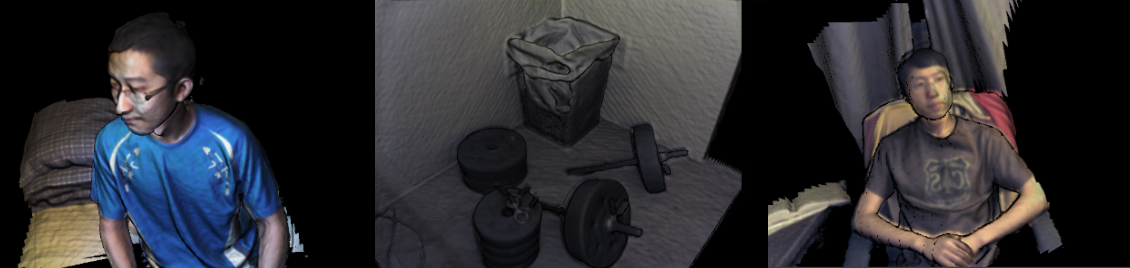
\includegraphics[width=\textwidth]{result.png}
\caption{\label{fig:shading}The color model under Phong shading}
\end{figure}

\section{Result}
In the experiment, our system was running on an Alienware m18x laptop with an Nvidia 680M graphics card attached with 2GB video memory. The volume resolution is set to $382^3$ with different voxel sizes. The result shows that, for most of the time, our system can maintain a 20 FPS rate even with 6 sub-texture rendering(as shown in Figure~\ref{fig:result}). 
We have noticed two minor problems in our system. The first problem is a drifting effect that occurs when the Kinect is facing a purely planar scene, our system is unstable in this case. The other problem is with colors: the location of the specular highlight is viewpoint-dependent, so when we change the viewpoint we are in effect accumulating highlights in many different locations, which can make the resulting model appear brighter than it really is. But overall, our system is robust across most scene settings and camera motions. Figure~\ref{fig:result} shows one snapshot taken from our system when running.

\section{Conclusions}
In this paper, we presented a new way to generate color models for real world objects by using the Kinect as a scanner, which may have lots of applications in computer game, animation, virtual environments and augmented reality (such as personal avatar generation, character designing etc). Also, the real-time performance feature of our system gives it the potential to be used as a tracking system in both virtual reality or robotics applications. But there are still problems that need to be solved: as mentioned in the result section, the drifting effect may be addressed by using an RGB feature based registration method in the future so the system can choose which registration method to use based on the scene configuration. A more challenging problem is the specular highlight problem. If we go a little bit further, we may want to find a way to extract material information from both the RGB and depth sensor. 

\begin{figure}[h!]
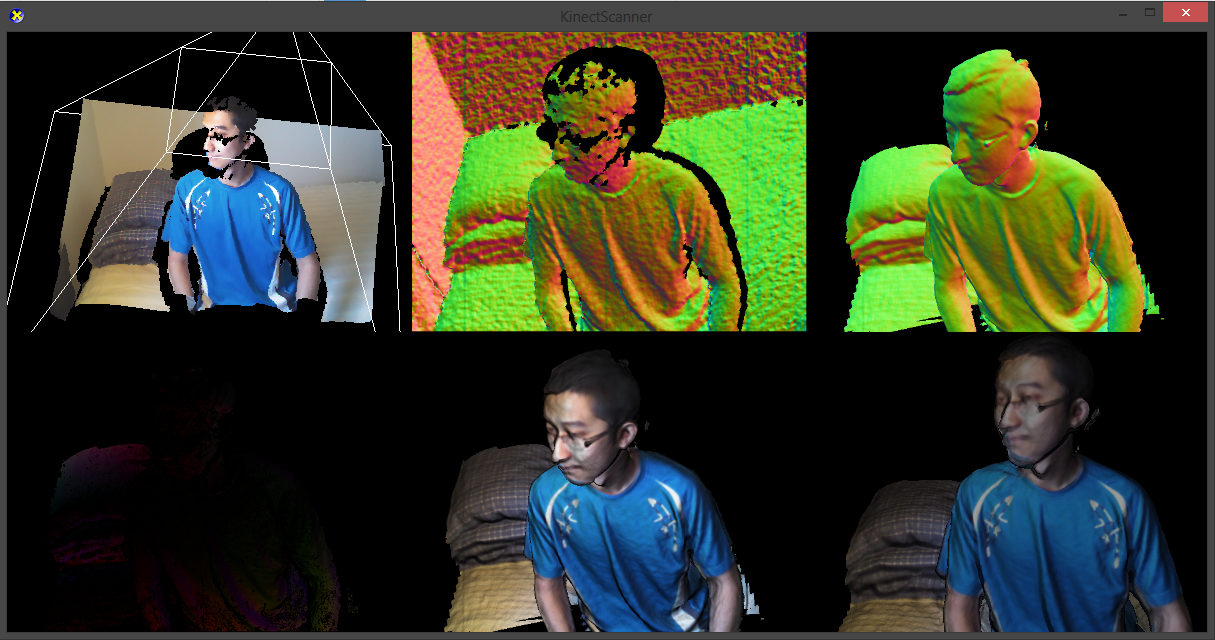
\includegraphics[width=\textwidth]{Bingzhe_Li_1.png}
\caption{\label{fig:result} The sub images from left to right, top to bottom show: live RGB-D visualization with the Kinect live pose; live Normal-Depth map from the Kinect; Normal-Depth map extracted from the TSDF; Error metric image; Phong shaded image from the Kinect's view; Phong shaded image from free camera's view }
\end{figure}

\bibliography{KinectScannerCollection.bib}
\bibliographystyle{IEEEtran}

\end{document}